%%*****************************************************************************
%% $Id$
%%*****************************************************************************
%% @author Gerd Neugebauer
%%-----------------------------------------------------------------------------
\chapter{Prerequisites}


\section{User Account at Berlios}

To commit changes to the repository you have to be enlisted as a
developer for \ExTeX. A first requirement for this is an account at
Berlios -- the hosting site. If you just want to read the sources then
you can use anonymous access.

To register at Berios use the page \url{http://developer.berlios.de/}
and select the item \menu{} on the upper left side. You will find
yourself in the registration page as shown in
figure~\ref{fig:berlios-register}. You will find your way through
easily.
\begin{figure}[htbp]
  \centering  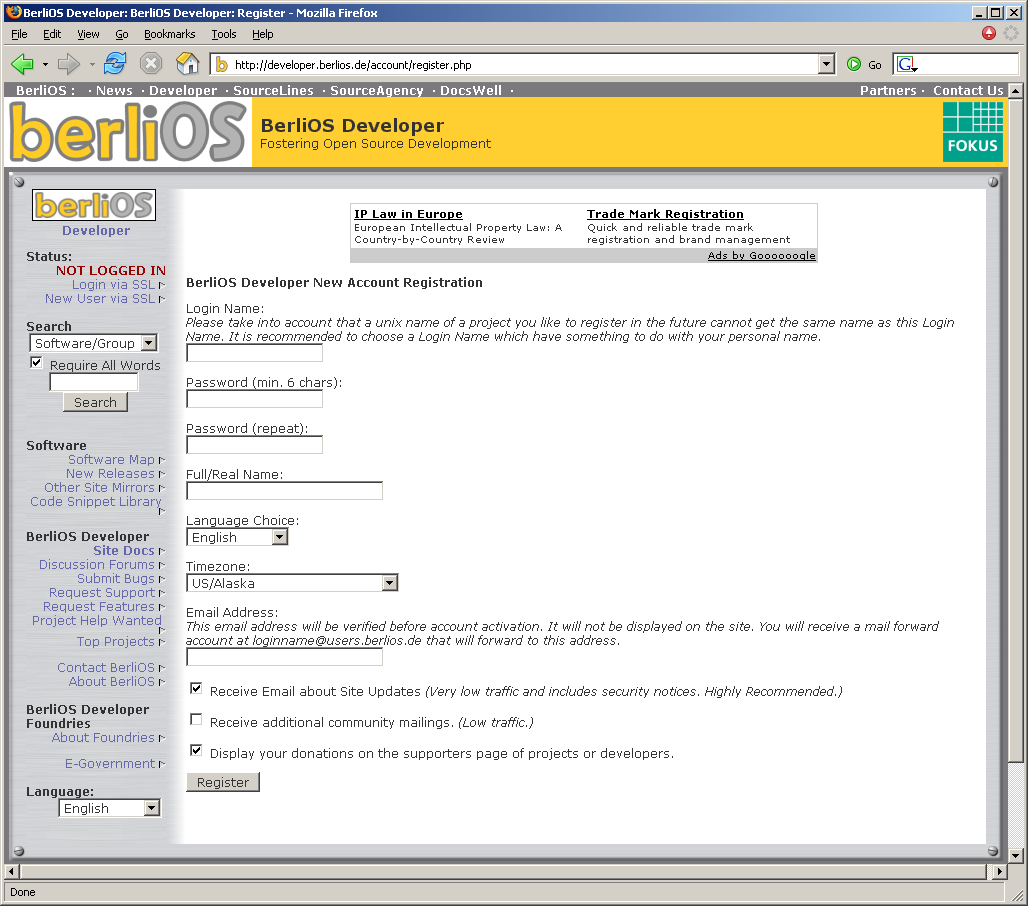
\includegraphics[scale=.33]{image/berlios-register}
  \caption{New Account at Berlios}\label{fig:berlios-register}
\end{figure}

When you have an account at Berlios you might be added to the
developers list of \ExTeX. This as to be done by one of the admins of
\ExTeX.


\section{Java}

You need to have Java 1.4.2\index{Java} or later installed on your
system. You can get Java for a several systems directly from
\url{java.sun.com}. Download and install it according to the
installation instructions for your environment.

To check that you have an appropriate Java on your path you can use
the command \texttt{java} with the argument \texttt{-version}. This
can be seen in the following listing:

\lstset{morecomment=[l]{\#}}%
\begin{lstlisting}{morecomment=[l][keywordstyle]{>}}
# java -version
java version "1.4.2_09"
Java(TM) 2 Runtime Environment, Standard Edition (build 1.4.2_09-b03)
Java HotSpot(TM) Client VM (build 1.4.2_09-b03, mixed mode)
#
\end{lstlisting}

Free Java implementations are currently not supported. They might
work, but the last time we checked it, GCJ didn't suffice. We would be
happy to have someone working on a compatibility layer for a free Java
implementation.


\section{TEXMF}

If you want to use more than the pure \ExTeX\ engine, fonts and macros
can be inherited from a texmf tree\index{texmf}. \ExTeX\ itself does
not contain a full texmf tree. It comes just with some rudimentary
files necessary for testing. Thus you should have installed a texmf
tree, e.g. from a \TeX Live\index{TeXlive@\TeX Live} installation.
This can be found on the \href{http://www.ctan.org}{Comprehensive
  \TeX\ Archive Network (CTAN)}\index{CTAN}.

There is no need to install the texmf tree in a special place. You
have to tell \ExTeX\ anyhow where it can be found. It is even possible
to work with several texmf trees.

One requirement for the texmf trees is that they have a file database
(\File{ls-R}). \ExTeX\ can be configured to work without it, but then
\ExTeX\ is deadly slow. Thus you do not really want to try this
alternative.

To use your texmf tree you should create a configuration file in your
home directory. On a Unix system the home directory is stored the
environment variable \verb|$HOME|. On a Windows system the home
directory is usually located under \verb|C:\WINDOWS\Profiles\|.  The
configuration file must have the name \File{.extex} (a little
intelligence test under Windows;-). It contains one line of the
following form

\begin{lstlisting}{}
texmf.tree=/usr/lib/texmf
\end{lstlisting}

The value should point to the location of the texmf tree. If you have
several texmf trees which need to be used you can put them into this
attribute by separating them by a platform-specific separator. This
separator is a colon (\verb|:|) under Unix and a semicolon (\verb|;|)
under Windows.


\section{CVS Client}

You need a CVS client installed. In the simplest case this is the
client build into the IDE Eclipse, or the command line version of cvs.


\section{A Command Line Interpreter}

For several tasks it is convenient to have a command line interpreter
at hand. On Unix this can be the (bourne, bash,\ldots) shell. On Windows
we recommend the Cygwin suite which contains the bash.


\section{Ant}

Ant is used throughout the whole buld system. For mpst purposes it is
sufficient to live with the files distributed. Nevertheless it might be
necessary to have ant installed and on the path for special tasks.


\section{Perl}

Perl is used to create the wae site. Thus it has to be installed for this
purpose. For the usual development it is not necesary to have Perl installed.


